\section{Quality Testing}

We now look at the solution quality. Although we used the unit testing library Catch2 to verify individual components, this does not suffice to verify that the entire application behaves correctly. This however can not be done with deterministic tests since \ac{SCITE} is a stochastic algorithm: Given different seeds, it produces different solutions which may or may not be perfect. We also could not implement \ac{ffSCITE} as a bit-exact copy of \ac{SCITE}, especially since we could not use the same \ac{URNG} as the reference implementation. We, therefore, needed to introduce a statistical test that verifies that given the same input, both \ac{SCITE} and \ac{ffSCITE} produce equivalent outputs. In this section, we discuss how we designed the test and what the results are.

\subsection{Methods}

Let $C$ be the set of considered cells, $G$ be the set of considered genes, and $d \in \{0,1,2\}^{|C| \times |G|}$ the input mutation data matrix. We model the output mutation trees of \ac{SCITE} and \ac{ffSCITE} given the inputs $C$, $G$, and $d$ as the random variables $T_\mathrm{SCITE}$ and $T_\mathrm{ffSCITE}$. We again work with log-likelihoods since the true likelihood scores for practically sized inputs are too close to 0 to express them using 64-bit floating-point numbers. Therefore, we intuitively want to find evidence for the statement $\mathbb{E} \log\Lambda_d(T_\mathrm{SCITE}) = \mathbb{E} \log\Lambda_d(T_\mathrm{ffSCITE})$. However, classical hypothesis tests are only able to provide evidence for inequality statements like $\mathbb{E} \log\Lambda_d(T_\mathrm{SCITE}) < \mathbb{E} \log\Lambda_d(T_\mathrm{ffSCITE})$. This is not what we aimed for and not what we claim. Therefore, we need a different approach.

In the field of clinical studies, non-inferiority and equivalence trials are a common tool. There, these kinds of trials ``are intended to show that the effect of a new treatment is not worse than that of an active control by more than a specified margin.'' \cite{snapinn2000noninferiority} Although there are some complications with using non-inferiority trails for drug testing as pointed out by Snapinn \cite{snapinn2000noninferiority}, these complications do not apply to our scenario. The exact procedure that we use is called \acf{TOST}, which was introduced by Schuirmann in 1987 \cite{schuirmann1987comparison} and it requires its designer to set an equivalence margin $\delta$, where absolute differences below this margin are considered negligible. Then, our alternative and null hypotheses are:
\begin{align*}
    H_1&: \mathbb{E} |\log\Lambda_d(T_\mathrm{SCITE}) - \log\Lambda_d(T_\mathrm{ffSCITE})| < \delta \\
    H_0&: \mathbb{E} |\log\Lambda_d(T_\mathrm{SCITE}) - \log\Lambda_d(T_\mathrm{ffSCITE})| \geq \delta \\
    &\Leftrightarrow \mathbb{E} \left(\log\Lambda_d(T_\mathrm{SCITE}) - \log\Lambda_d(T_\mathrm{ffSCITE})\right) \leq - \delta \vee \mathbb{E} \left(\log\Lambda_d(T_\mathrm{SCITE}) - \log\Lambda_d(T_\mathrm{ffSCITE})\right) \geq \delta
\end{align*}
Once our hypotheses are established, we can execute a one-sided t-test for each half of $H_0$ and if both fail, we have provided evidence for the equivalence for \ac{ffSCITE} and \ac{SCITE}.

Intuitively, we want to pick $\delta$ as close to 0 as possible, but we still want to provide a reasonable margin. A natural choice for $\delta$ might be the maximum likelihood difference from one chain step to the next. If ffSCITE were equivalent to SCITE within this margin, it would mean that ffSCITE may have only missed the last chain step to the optimal solution, which one could deem as negligible. However, the effects of a chain step may be chaotic since the cell-node attachments are recomputed and might change after every operation. These attachment changes not only depend on the mutation tree, but also the error probabilities and the observed mutation data. As of this writing, we do not have enough understanding of a chain step's effect on the state likelihood, and we also did not have the time to develop it. Therefore, we decided to work on the mutation matrix level instead. This is also justified by the fact that we have assigned the likelihood score in definition \ref{def:likelihood} to mutation matrices, not to mutation trees. These are only a tool to ease the proposal of mutation matrices. Therefore, we have decided to set our $\delta$ to the maximum log-likelihood difference induced by a bit-flip, the smallest logical difference between two bit matrices. According to lemma \ref{lem:bitflip}, this is 
\begin{align*}
    \delta :=\max\{|\log(\alpha) - \log(1-\beta)|, |\log(\beta) - \log(1-\alpha)|\}
\end{align*}
where $\alpha$ and $\beta$ are the probabilities for false positives and negatives, respectively.

\begin{lemma}
    \label{lem:bitflip}
    Let $C$ be the set of considered cells, $G$ be the set of considered genes, $d \in \{0,1,2\}^{|C| \times |G|}$, and $e, e' \in \{0,1\}^{|C| \times |G|}$ where $e$ is arbitrary and $e'$ is defined as:
    \begin{align*}
        e'_{c,g} &:= \begin{cases}
            \overline{e_{c,g}} & c = x \wedge g = y \\
            e_{c,g} & \text{else}
        \end{cases}
    \end{align*}
    for some $x \in C$, $y \in G$. In other words, $e'$ is a version of $e$ where the bit at position $(x,y)$ is flipped. Let also $\alpha, \beta \in [0,1]$ be the probabilities of false positives and negatives, respectively. Then, we have:
    \begin{align*}
        |\log\Lambda_d(e) - \log\Lambda_d(e')| &\leq \max\{|\log(\alpha) - \log(1-\beta)|, |\log(\beta) - \log(1-\alpha)|\}
    \end{align*}
    where $\Lambda_d$ is the likelihood function of definition \ref{def:likelihood}. In other words, the difference in log-likelihood induced by a single bit flip is equal to or less than $\max\{|\log(\alpha) - \log(1-\beta)|, |\log(\beta) - \log(1-\alpha)|\}$.
\end{lemma}

\begin{proof}
    First of all, we should remark that we have
    \begin{align*}
        \log\Lambda_d(e) &= \sum_{c \in C} \sum_{g \in G} \log\lambda(d_{c,g}, e_{c,g}) \\
        \Rightarrow |\log\Lambda_d(e) - \log\Lambda_d(e')| &= |\log\lambda(d_{x,y}, e_{x,y}) - \log\lambda(d_{x,y}, e'_{x,y})| \\
        &= |\log\lambda(d_{x,y}, e_{x,y}) - \log\lambda(d_{x,y}, \overline{e_{x,y}})|
    \end{align*}
    If we have $d_{x,y} = 2$, we therefore have
    \begin{align*}
        |\log\Lambda_d(e) - \log\Lambda_d(e')| &= |\log(1) - \log(1)| = 0
    \end{align*}
    Now, one can consider all combinations for $d_{x,y}$ and $e_{x,y}$ to find that we either have 
    \begin{align*}
        |\log\Lambda_d(e) - \log\Lambda_d(e')| = |\log(1-\alpha) - \log(\beta)|
    \end{align*}
    or
    \begin{align*}
        |\log\Lambda_d(e) - \log\Lambda_d(e')| = |\log(1-\beta) - \log(\alpha)|
    \end{align*}
    and therefore
    \begin{align*}
        |\log\Lambda_d(e) - \log\Lambda_d(e')| &\leq \max\{|\log(\alpha) - \log(1-\beta)|, |\log(\beta) - \log(1-\alpha)|\}
    \end{align*}
\end{proof}

Let us summarize our quality testing method: First, we have randomly generated 64 observed mutation data matrices considering 64 cells and 63 genes, with a probability of $\alpha := 10^{-6}$ for false positives, $\beta := 0.25$ for false negatives, and $0.25$ for missing data. Then, we ran 6 chains á 1,000,000 steps on these mutation data matrices, using both \ac{SCITE} and \ac{ffSCITE}, and stored the resulting max-likelihood mutation trees. This input size of 64 cells and 63 genes is the maximum our build of \ac{ffSCITE} can support. We chose the number of input sets, chains, and steps as a compromise between expressiveness and execution time since we wanted to run the same experiment multiple times during development to continuously check our design. The error probabilities are however arbitrary since we did not have realistic numbers available or the time to research them. After the execution was completed, we used a Python script to compute the differences in log-likelihood produced by \ac{SCITE} and \ac{ffSCITE} for the same inputs and used SciPy to run one-sided t-tests against the parts of our null-hypothesis with a significance level of 0.01. Therefore, the significance level of the entire test is 0.02.

\subsection{Results}

Out of the 64 inputs, \ac{SCITE} and \ac{ffSCITE} achieved the same likelihoods for 47 inputs. \ac{ffSCITE} scored better in 10 cases, and \ac{SCITE} scored better in 7 cases. Interestingly, all encountered differences are multiples of our $\delta$, which is defined as the maximum difference induced by a bit-flip. Therefore, we plotted the number of outputs with a certain log-likelihood difference in multiples of $\delta$ or bit-flips in figure \ref{fig:likelihood_differences}. Another notable finding is that \ac{SCITE} and \ac{ffSCITE} never deviate by more than two bit-flips and the mean difference between \ac{SCITE}'s and \ac{ffSCITE}'s log-likelihood score is $0.65$. Lastly, the p-value for the test of $\mathbb{E} \left(\log\Lambda_d(T_\mathrm{SCITE}) - \log\Lambda_d(T_\mathrm{ffSCITE})\right) \leq - \delta$ is $p_- \approx 9.47 \cdot 10^{-21}$ and the p-value for the test of $\mathbb{E} \left(\log\Lambda_d(T_\mathrm{SCITE}) - \log\Lambda_d(T_\mathrm{ffSCITE})\right) \geq \delta$ is $p_+ \approx 7.87 \cdot 10^{-19}$. Since both of them are lower than our significance level of $0.01$, we have to reject $H_0$ and have provided evidence that \ac{ffSCITE} and \ac{SCITE} produce solutions of equivalent quality.

\begin{figure}
    \centering
    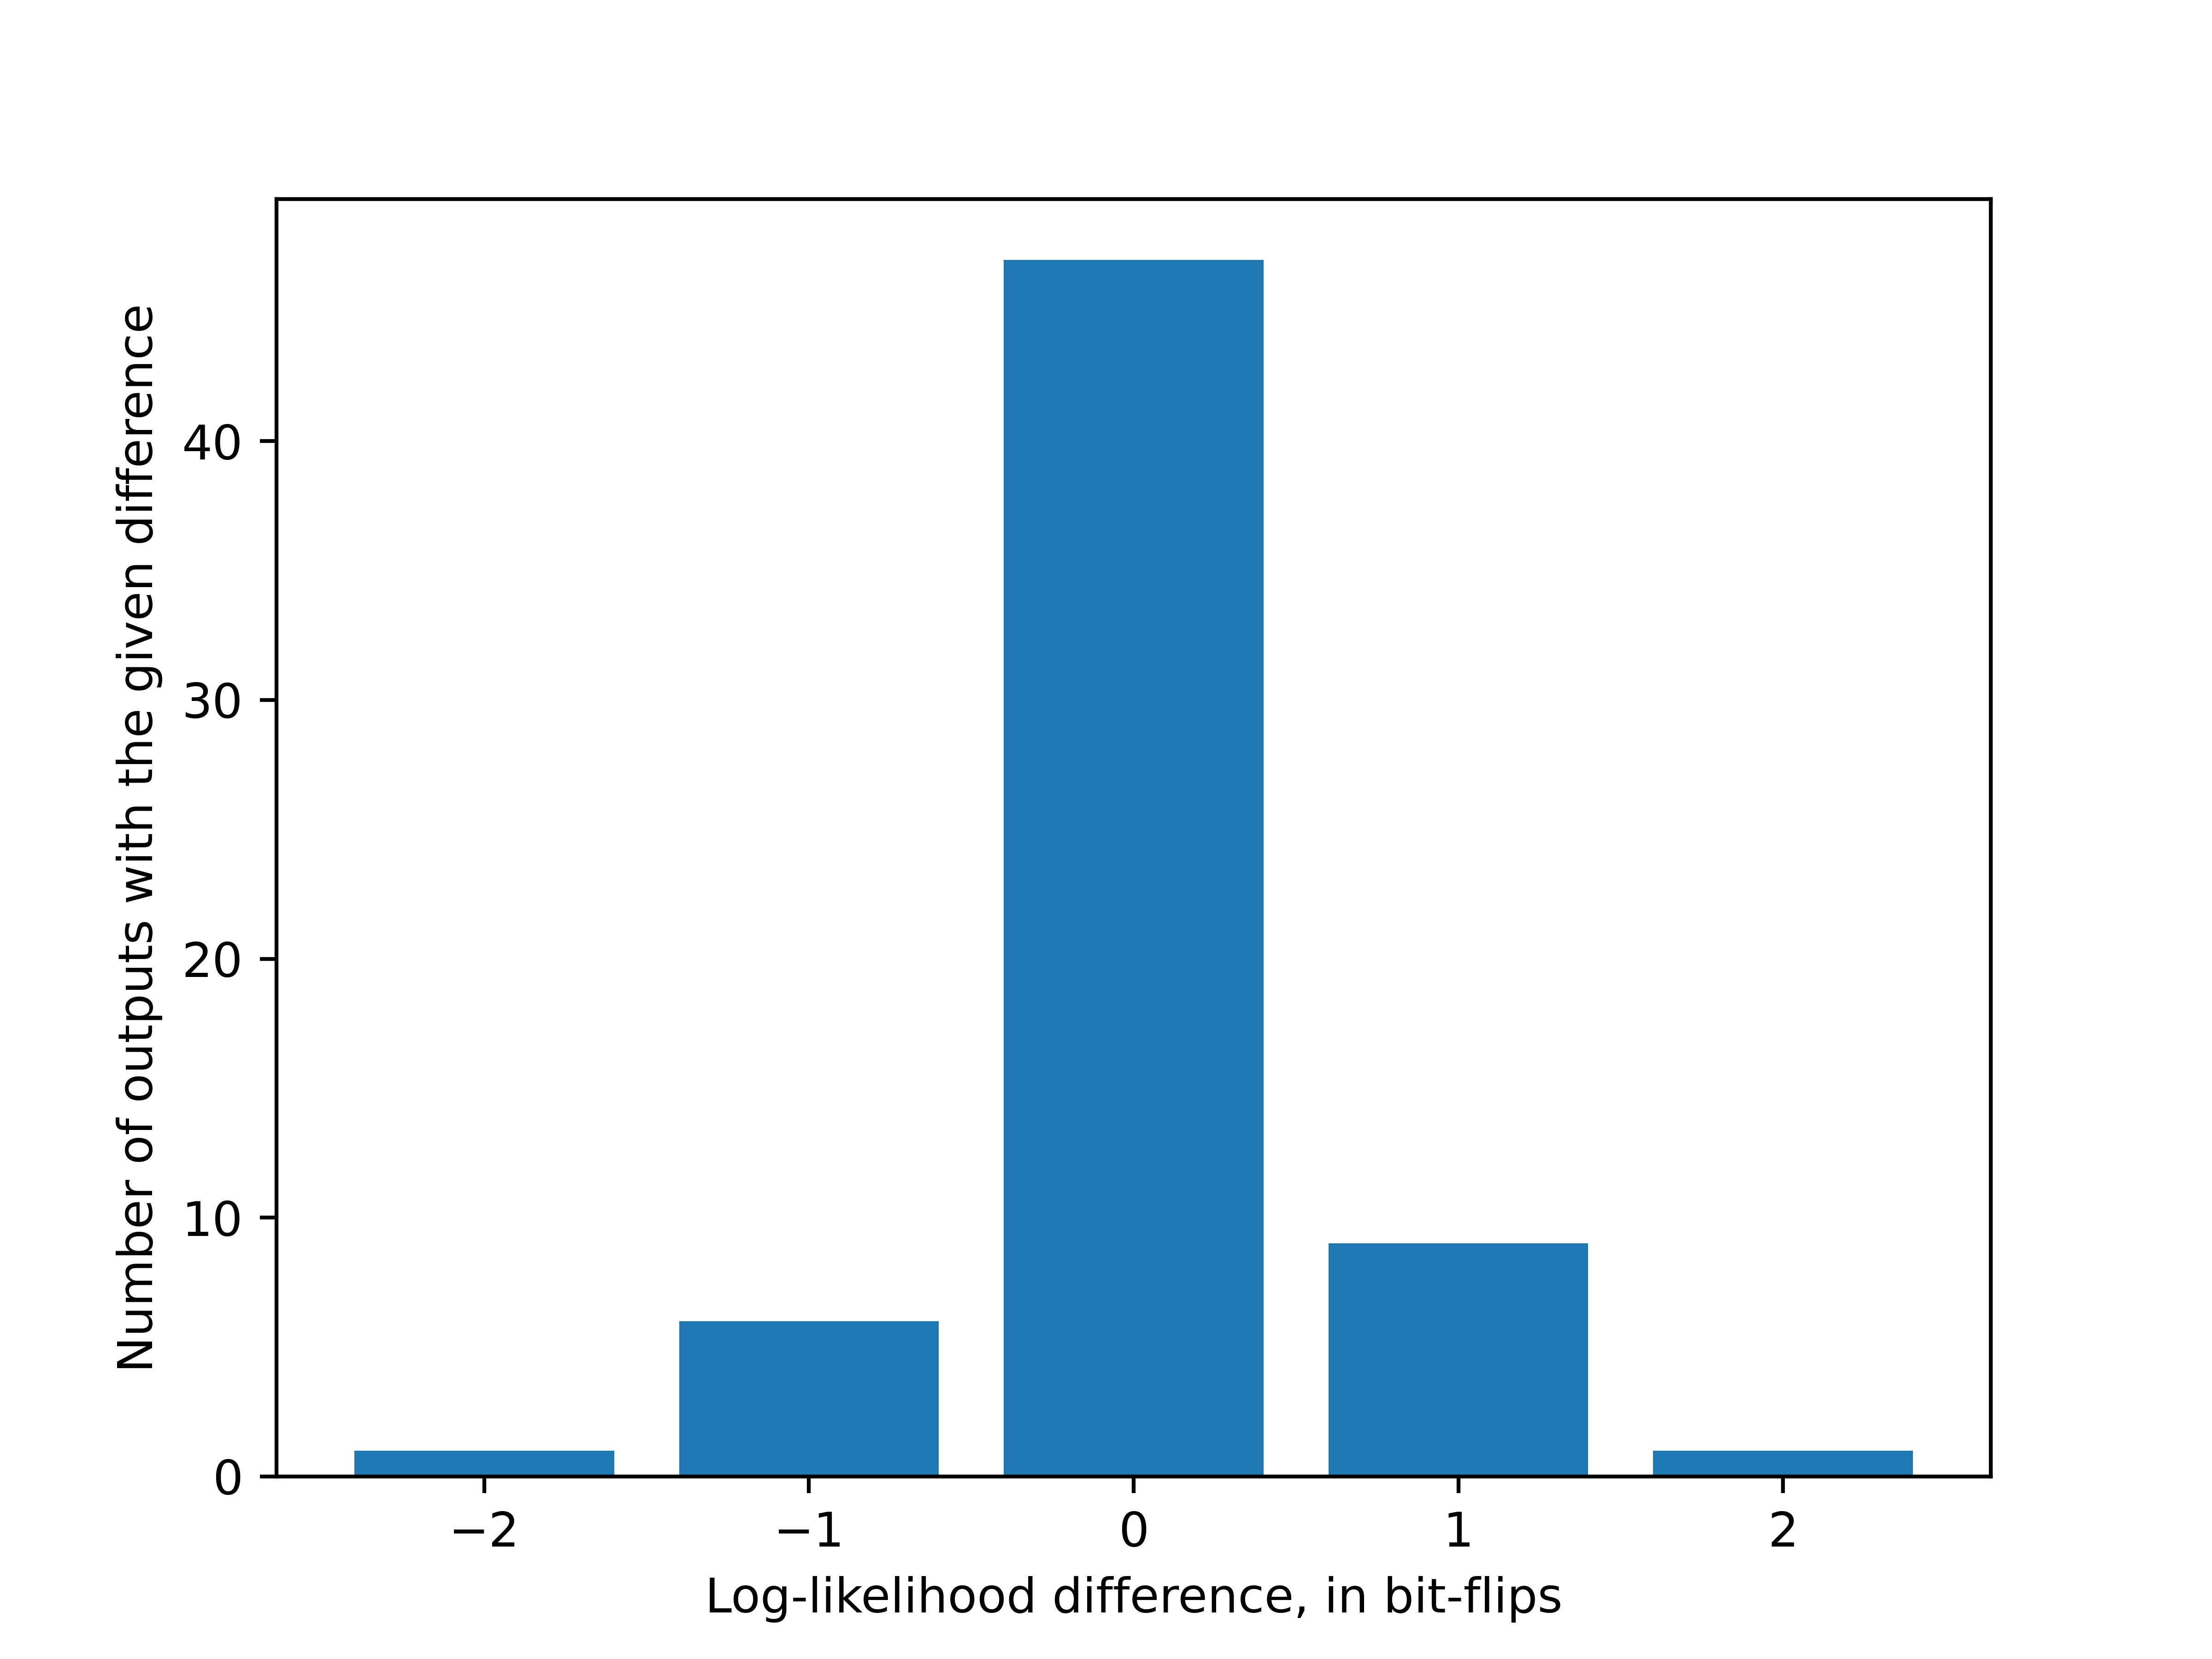
\includegraphics[width=0.75\textwidth]{figures/likelihood_differences.png}
    \caption{Accumulated differences in log-likelihood between solutions provided by \ac{SCITE} and \ac{ffSCITE}. A positive difference means that \ac{ffSCITE} has provided a better solution than \ac{SCITE}, and a negative difference means the opposite.}
    \label{fig:likelihood_differences}
\end{figure}